\documentclass{article}

\usepackage{rotating}
\usepackage[margin=1in]{geometry}
\usepackage{booktabs}
\usepackage{caption, subcaption}
\usepackage{hyperref}

\begin{document}

\begin{sidewaystable}

\caption{Replication of Ouazad and Kahn (2022) using the LLPW Suggested Data Cleaning Rules}

\begin{center}
\begingroup
\centering
\begin{tabular}{lccccccccc}
   \tabularnewline \midrule \midrule
   Dependent Variables: & \multicolumn{3}{c}{approved} & \multicolumn{3}{c}{originated} & \multicolumn{3}{c}{securitized}\\
                                                              & 20\%           & 10\%           & 5\%            & 20\%          & 10\%           & 5\%           & 20\%         & 10\%          & 5\% \\    
   Model:                                                     & (1)            & (2)            & (3)            & (4)           & (5)            & (6)           & (7)          & (8)           & (9)\\  
   \midrule
   \emph{Variables}\\
   Below Conforming Limit  $\times$ Treated $\times$ Time -4  & 0.0034         & 0.0129         & 0.0203         & -0.0029       & 0.0204         & 0.0497$^{**}$ & 0.0103       & 0.0081        & 0.0170\\   
                                                              & (0.0081)       & (0.0137)       & (0.0187)       & (0.0087)      & (0.0152)       & (0.0174)      & (0.0185)     & (0.0159)      & (0.0171)\\   
   Below Conforming Limit $\times$ Treated $\times$ Time -3   & -0.0072        & 0.0058         & 0.0068         & -0.0086       & 0.0156         & 0.0306        & 0.0004       & -0.0234       & -0.0220\\   
                                                              & (0.0096)       & (0.0067)       & (0.0184)       & (0.0123)      & (0.0118)       & (0.0283)      & (0.0142)     & (0.0198)      & (0.0315)\\   
   Below Conforming Limit $\times$ Treated $\times$ Time -2   & -0.0089        & -0.0093        & -0.0044        & -0.0060       & -0.0059        & -0.0002       & 0.0010       & -0.0152       & -0.0233\\   
                                                              & (0.0059)       & (0.0059)       & (0.0058)       & (0.0067)      & (0.0056)       & (0.0080)      & (0.0144)     & (0.0138)      & (0.0158)\\   
   Below Conforming Limit $\times$ Treated $\times$ Time +0   & -0.0079        & 0.0018         & 0.0040         & -0.0120       & 0.0004         & 0.0068        & 0.0022       & -0.0016       & 0.0070\\   
                                                              & (0.0055)       & (0.0093)       & (0.0084)       & (0.0070)      & (0.0127)       & (0.0135)      & (0.0088)     & (0.0103)      & (0.0112)\\   
   Below Conforming Limit $\times$ Treated $\times$ Time +1   & 0.0058         & 0.0235$^{**}$  & 0.0240$^{***}$ & 0.0009        & 0.0177         & 0.0282$^{**}$ & -0.0017      & -0.0068       & 0.0177\\   
                                                              & (0.0067)       & (0.0091)       & (0.0080)       & (0.0102)      & (0.0120)       & (0.0100)      & (0.0161)     & (0.0193)      & (0.0222)\\   
   Below Conforming Limit $\times$ Treated $\times$ Time +2   & 0.0066         & 0.0229$^{**}$  & 0.0349$^{***}$ & 0.0118        & 0.0142         & 0.0369$^{**}$ & -0.0171      & -0.0233       & -0.0076\\   
                                                              & (0.0055)       & (0.0081)       & (0.0086)       & (0.0102)      & (0.0109)       & (0.0128)      & (0.0155)     & (0.0202)      & (0.0225)\\   
   Below Conforming Limit $\times$ Treated $\times$ Time +3   & 0.0372$^{***}$ & 0.0515$^{***}$ & 0.0550$^{***}$ & 0.0328$^{**}$ & 0.0478$^{***}$ & 0.0495$^{**}$ & 0.0354$^{*}$ & 0.0425$^{**}$ & 0.0610$^{**}$\\   
                                                              & (0.0078)       & (0.0095)       & (0.0158)       & (0.0125)      & (0.0108)       & (0.0179)      & (0.0197)     & (0.0198)      & (0.0282)\\   
   Below Conforming Limit $\times$ Treated $\times$ Time +4   & 0.0283         & 0.0276         & 0.0272         & 0.0060        & 0.0142         & 0.0143        & 0.0729       & 0.0902$^{*}$  & 0.1269$^{**}$\\   
                                                              & (0.0162)       & (0.0182)       & (0.0314)       & (0.0126)      & (0.0139)       & (0.0366)      & (0.0474)     & (0.0496)      & (0.0546)\\   
   \midrule
   \emph{Fixed-effects}\\
   Year                                                       & Yes            & Yes            & Yes            & Yes           & Yes            & Yes           & Yes          & Yes           & Yes\\  
   5-digit Zip Code                                           & Yes            & Yes            & Yes            & Yes           & Yes            & Yes           & Yes          & Yes           & Yes\\  
   Disaster                                                   & Yes            & Yes            & Yes            & Yes           & Yes            & Yes           & Yes          & Yes           & Yes\\  
   \midrule
   \emph{Fit statistics}\\
   Observations                                               & 2,572,574      & 1,436,349      & 897,489        & 2,572,574     & 1,436,349      & 897,489       & 2,835,727    & 1,590,131     & 1,004,977\\  
   R$^2$                                                      & 0.05960        & 0.06287        & 0.06359        & 0.06176       & 0.06362        & 0.06391       & 0.12886      & 0.10934       & 0.08322\\  
   Within R$^2$                                               & 0.00403        & 0.00433        & 0.00437        & 0.00342       & 0.00352        & 0.00349       & 0.08110      & 0.06046       & 0.03531\\  
   \midrule \midrule
   \multicolumn{10}{l}{\emph{Clustered (5-digit Zip Code \& year) standard-errors in parentheses}}\\
   \multicolumn{10}{l}{\emph{Signif. Codes: ***: 0.01, **: 0.05, *: 0.1}}\\
\end{tabular}
\par\endgroup

\end{center}

\end{sidewaystable}

\clearpage
\pagebreak

\begin{sidewaystable}

\caption{Replication of Ouazad and Kahn (2022) – Narrower Window}
\begingroup
\centering
\begin{tabular}{lccccccccc}
   \tabularnewline \midrule \midrule
   Dependent Variables: & \multicolumn{3}{c}{approved} & \multicolumn{3}{c}{originated} & \multicolumn{3}{c}{securitized}\\
                                                              & 4\%                    & 3\%            & 2\%           & 4\%           & 3\%            & 2\%           & 4\%           & 3\%           & 2\% \\    
   Model:                                                     & (1)                    & (2)            & (3)           & (4)           & (5)            & (6)           & (7)           & (8)           & (9)\\  
   \midrule
   \emph{Variables}\\
   Below Conforming Limit $\times$ Time -4 $\times$ Treated   & 0.0151                 & 0.0340$^{**}$  & 0.0478$^{*}$  & 0.0469$^{**}$ & 0.0713$^{***}$ & 0.0692$^{**}$ & 0.0371$^{*}$  & 0.0484$^{**}$ & 0.0282\\   
                                                              & (0.0141)               & (0.0138)       & (0.0262)      & (0.0202)      & (0.0226)       & (0.0316)      & (0.0181)      & (0.0217)      & (0.0311)\\   
   Below Conforming Limit $\times$ Treated $\times$ Time -3   & 0.0058                 & 0.0144         & 0.0055        & 0.0248        & 0.0302         & 0.0160        & -0.0127       & -0.0123       & -0.0092\\   
                                                              & (0.0190)               & (0.0202)       & (0.0252)      & (0.0350)      & (0.0341)       & (0.0370)      & (0.0303)      & (0.0345)      & (0.0368)\\   
   Below Conforming Limit $\times$ Treated $\times$ Time -2   & -0.0037                & 0.0013         & -0.0014       & -0.0010       & 0.0062         & 0.0013        & -0.0172       & -0.0199       & -0.0206\\   
                                                              & (0.0027)               & (0.0099)       & (0.0132)      & (0.0148)      & (0.0156)       & (0.0211)      & (0.0175)      & (0.0191)      & (0.0193)\\   
   Below Conforming Limit $\times$ Treated $\times$ Time +0   & $-7.45\times 10^{-5}$  & 0.0014         & -0.0029       & -0.0024       & 0.0012         & -0.0114       & 0.0130        & 0.0058        & 0.0044\\   
                                                              & (0.0095)               & (0.0138)       & (0.0131)      & (0.0187)      & (0.0226)       & (0.0256)      & (0.0148)      & (0.0171)      & (0.0236)\\   
   Below Conforming Limit $\times$ Treated $\times$ Time +1   & 0.0272$^{***}$         & 0.0370$^{***}$ & 0.0369$^{**}$ & 0.0316$^{*}$  & 0.0479$^{**}$  & 0.0462        & 0.0341        & 0.0330        & 0.0385\\   
                                                              & (0.0033)               & (0.0105)       & (0.0133)      & (0.0167)      & (0.0187)       & (0.0273)      & (0.0260)      & (0.0241)      & (0.0264)\\   
   Below Conforming Limit $\times$ Treated $\times$ Time +2   & 0.0430$^{***}$         & 0.0473$^{*}$   & 0.0506$^{*}$  & 0.0362$^{**}$ & 0.0403         & 0.0348        & 0.0033        & 0.0044        & 0.0201\\   
                                                              & (0.0135)               & (0.0224)       & (0.0251)      & (0.0166)      & (0.0233)       & (0.0362)      & (0.0265)      & (0.0240)      & (0.0222)\\   
   Below Conforming Limit $\times$ Treated $\times$ Time +3   & 0.0575$^{***}$         & 0.0606$^{***}$ & 0.0626$^{**}$ & 0.0558$^{**}$ & 0.0643$^{**}$  & 0.0530        & 0.0732$^{**}$ & 0.0707$^{**}$ & 0.0917$^{**}$\\   
                                                              & (0.0167)               & (0.0145)       & (0.0213)      & (0.0234)      & (0.0286)       & (0.0304)      & (0.0285)      & (0.0310)      & (0.0335)\\   
   Below Conforming Limit $\times$ Treated $\times$ Time +4   & 0.0252                 & 0.0250         & 0.0314        & 0.0027        & -0.0021        & 0.0032        & 0.1440$^{**}$ & 0.1506$^{**}$ & 0.1872$^{***}$\\   
                                                              & (0.0349)               & (0.0388)       & (0.0420)      & (0.0419)      & (0.0461)       & (0.0489)      & (0.0543)      & (0.0550)      & (0.0617)\\   
   \midrule
   \emph{Fixed-effects}\\
   Year                                                       & Yes                    & Yes            & Yes           & Yes           & Yes            & Yes           & Yes           & Yes           & Yes\\  
   5-digit Zip Code                                           & Yes                    & Yes            & Yes           & Yes           & Yes            & Yes           & Yes           & Yes           & Yes\\  
   Disaster                                                   & Yes                    & Yes            & Yes           & Yes           & Yes            & Yes           & Yes           & Yes           & Yes\\  
   \midrule
   \emph{Fit statistics}\\
   Observations                                               & 755,908                & 671,790        & 574,089       & 755,908       & 671,790        & 574,089       & 854,091       & 762,323       & 657,406\\  
   R$^2$                                                      & 0.06524                & 0.06536        & 0.06503       & 0.06473       & 0.06380        & 0.06258       & 0.08069       & 0.07057       & 0.06106\\  
   Within R$^2$                                               & 0.00542                & 0.00523        & 0.00557       & 0.00442       & 0.00424        & 0.00443       & 0.03302       & 0.02500       & 0.01970\\  
   \midrule \midrule
   \multicolumn{10}{l}{\emph{Clustered (5-digit Zip Code \& year) standard-errors in parentheses}}\\
   \multicolumn{10}{l}{\emph{Signif. Codes: ***: 0.01, **: 0.05, *: 0.1}}\\
\end{tabular}
\par\endgroup


\begin{center}

\end{center}

\end{sidewaystable}

\clearpage
\pagebreak

\begin{table}

\caption{NaN values for the 'high cost' Dummy Variable: Only in the Sample for LLPW Table 7}

\emph{This Figure analyzes the 'high\_cost' variable in Ouazad and Kahn (2022) (named highcost), in the sample for Table 5 of LLPW, in the sample Table 7 of LLPW. This is verifiable in the RFS Dataverse of LLPW posted in August 2023 and the RFS Dataverse of Ouazad and Kahn (2022) posted in December 2021. In LLPW, the 'high\_cost' variable is a key part of the match of the sample with high cost conforming loan limits.}

\begin{center}
% latex table generated in R 4.3.2 by xtable 1.8-4 package
% Tue Aug 27 18:28:04 2024
\begin{tabular}{lccc}
  \hline
Sample & NaN & 0 & 1 \\ 
  \hline
OK (2022) &   0 & 1282735 & 524582 \\ 
  LPW (2023) Table 5 &   0 & 2552216 & 1181257 \\ 
  LPW (2023) Table 7 & 32030 & 2545637 & 2599249 \\ 
   \hline
\end{tabular}


\end{center}

\emph{NaN values appear in the sample for Table 7. This is the Table that does not find the results of Ouazad and Kahn (2022).}

\end{table}

\begin{table}
\caption{LLPW Table 7 -- NaN values for the 'high cost' Dummy Variable, by Action Taken}

\emph{This Figure analyzes the 'high\_cost' variable of the sample for Table 7 of LLPW. This is verifiable in the RFS Dataverse of LLPW. The 'high\_cost' variable is a key part of the match of the sample with high cost conforming loan limits.}

\begin{center}
% latex table generated in R 4.3.2 by xtable 1.8-4 package
% Tue Aug 27 18:28:03 2024
\begin{tabular}{llccc}
  \hline
Action Taken & Description & NaN & 0 & 1 \\ 
  \hline
1 & Loan originated & 19991 & 1613850 & 1598895 \\ 
  2 & Application approved but not accepted & 1942 & 143029 & 161299 \\ 
  3 & Application denied & 3764 & 215109 & 229445 \\ 
  6 & Loan purchased by the institution & 6333 & 573649 & 609610 \\ 
   \hline
\end{tabular}


\end{center}

\end{table}

\begin{table}
\caption{LLPW Table 7 -- NaN values for the 'high cost' Dummy Variable by State}
\begin{center}
% latex table generated in R 4.3.2 by xtable 1.8-4 package
% Tue Aug 27 18:28:02 2024
\begin{tabular}{llccc}
  \hline
State FIPS Code & State Name & NaN & 0 & 1 \\ 
  \hline
01 & Alabama & 737 & 63614 &   0 \\ 
  09 & Connecticut &   0 & 101043 & 88305 \\ 
  10 & Delaware &   0 & 26619 &   0 \\ 
  12 & Florida & 15623 & 694424 & 22712 \\ 
  13 & Georgia & 1591 & 339425 & 440 \\ 
  22 & Louisiana & 766 & 46633 &   0 \\ 
  23 & Maine & 252 & 19268 &   0 \\ 
  24 & Maryland & 157 & 16685 & 371999 \\ 
  25 & Massachusetts &  35 & 69800 & 424192 \\ 
  28 & Mississippi & 773 & 18380 &   0 \\ 
  33 & New Hampshire & 286 & 24960 & 21529 \\ 
  34 & New Jersey &  16 & 88302 & 496638 \\ 
  36 & New York & 724 & 47997 & 647583 \\ 
  37 & North Carolina & 1291 & 253490 & 185 \\ 
  44 & Rhode Island &  79 &   0 & 32724 \\ 
  45 & South Carolina & 409 & 97329 &   0 \\ 
  48 & Texas & 2187 & 610148 &   0 \\ 
  51 & Virginia & 7104 & 27520 & 492942 \\ 
   \hline
\end{tabular}


\end{center}
    
\end{table}

\clearpage
\pagebreak

\begin{figure}
    
\caption{LLPW Table 7 -- NaN values for the 'high cost' Dummy Variable Bunch at the Conforming Loan Limit}

\emph{This Figure analyzes the presence of NaNs in the 'high\_cost' variable of the sample for Table 7 of LLPW. This is verifiable in the RFS Dataverse of LLPW. In LLPW, the 'high\_cost' variable is a key part of the match of the sample with high cost conforming loan limits.}

\begin{center}
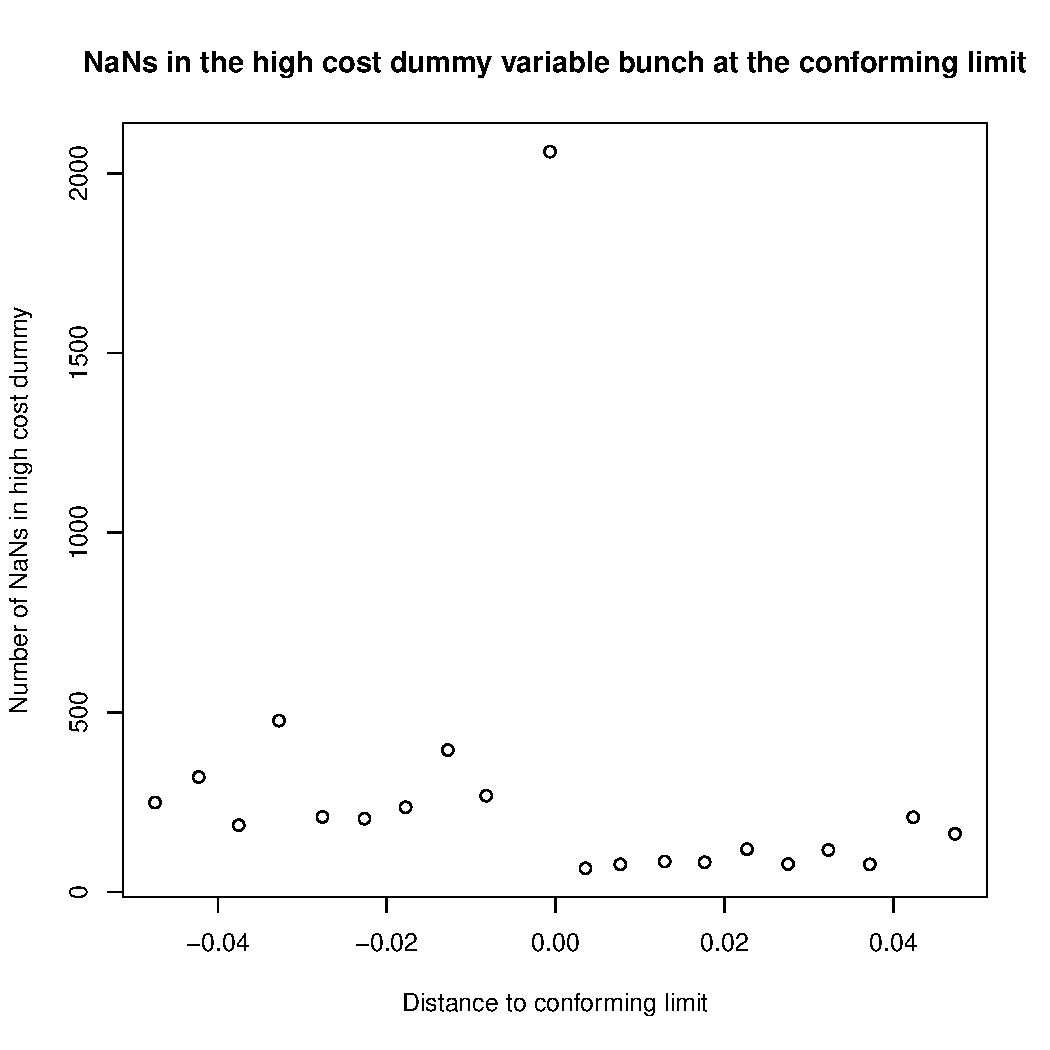
\includegraphics[scale = 0.5]{02_evidence_of_data_errors_in_LPW_2024_Table_7/figures/nans_in_high_cost_dummy_bunching.pdf}
\end{center}

\end{figure}

\clearpage
\pagebreak

\begin{table}
    
\caption{ZIPs Arbitrarily Excluded in the RFS Dataverse Code of LLPW (2024) Are Present in Ouazad and Kahn (2022)} 

Lines 140--143 of the 02\_generateRegressionSample.m of LLPW arbitrarily exclude 20 ZIP codes. The code claims that these ZIP codes are excluded in Ouazad and Kahn (2022). The RFS Dataverse of Ouazad and Kahn (2022) dated December 6, 2021, shows that these observations are present in the sample and are part of the treatment group. Column 4 shows which hurricane hit the ZIP code in Ouazad and Kahn's (2022) sample.

\bigskip

\begin{center}
    % latex table generated in R 4.3.2 by xtable 1.8-4 package
% Tue Aug 27 21:46:35 2024
\begin{tabular}{cccc}
  \hline
5-digit ZIPs Excluded by LPW & Treated in OK (2022) & State FIPS & Hurricane in OK (2022) \\ 
  \hline
70615 & Yes & 22 & RITA 2005 \\ 
  77702 & Yes & 48 & RITA 2005 \\ 
  21085 & Yes & 24 & SANDY 2012 \\ 
  11096 & Yes & 36 & SANDY 2012 \\ 
  19703 & Yes & 10 & SANDY 2012 \\ 
  10474 & Yes & 36 & SANDY 2012 \\ 
  21017 & Yes & 24 & SANDY 2012 \\ 
  10303 & Yes & 36 & SANDY 2012 \\ 
  70094 & Yes & 22 & KATRINA 2005 \\ 
  39576 & Yes & 28 & KATRINA 2005 \\ 
  70094 & Yes & 22 & GUSTAV 2008 \\ 
  77702 & Yes & 48 & IKE 2008 \\ 
  77530 & Yes & 48 & IKE 2008 \\ 
  77480 & Yes & 48 & IKE 2008 \\ 
  77058 & Yes & 48 & IKE 2008 \\ 
  77591 & Yes & 48 & IKE 2008 \\ 
  77506 & Yes & 48 & IKE 2008 \\ 
  23664 & Yes & 51 & IRENE 2011 \\ 
  23602 & Yes & 51 & IRENE 2011 \\ 
  23661 & Yes & 51 & IRENE 2011 \\ 
  23314 & Yes & 51 & IRENE 2011 \\ 
  27981 & Yes & 37 & IRENE 2011 \\ 
   \hline
\end{tabular}


\end{center}

\bigskip

The table below shows the average distance (in logs) to the conforming loan limit of the loans in these excluded ZIPs. These ZIPs are more likely to have conforming loans.

\bigskip

\begin{center}
    % latex table generated in R 4.3.2 by xtable 1.8-4 package
% Tue Aug 27 21:46:50 2024
\begin{tabular}{lcccccc}
  \hline
Sample & Min. & 1st Qu. & Median & Mean & 3rd Qu. & Max. \\ 
  \hline
Excluded ZIPs & -0.10 & -0.08 & -0.04 & -0.03 & 0.01 & 0.10 \\ 
  Rest of the sample & -0.11 & -0.06 & -0.01 & -0.02 & 0.00 & 0.10 \\ 
   \hline
\end{tabular}


\end{center}

\end{table}

\clearpage
\pagebreak

\begin{table}
\caption{The Independent Replication of LLPW, Table 8, has Non-Mutually Exclusive Time Dummies}

\emph{The independent replication package (not Tables 5--7) was accessed in April 2023 and is stored on our cloud at \url{https://tinyurl.com/yy7s7b9c}. Since the RFS Dataverse of LLPW does not include the code for Table 8, we assume this is consistent with it. This table presents, for the treatment group only, the sum of the indicator variables for the number of years relative to the hurricane. In a well-designed event study, each treated observation should have only one time dummy variable equal to 1. Except for the reference time period (e.g. $-1$). In contrast, in the independent replication, more than 93,000 observations are in the treatment but have no corresponding time dummy. And more than 6,200 observations have multiple time dummies equal to 1 at the same time. There is no dummy variable for times before $-4$ and no dummy variable for times after $+4$. }

\begin{center}
\begin{tabular}{lcccc}
    \toprule
    & \multicolumn{4}{c}{$\sum_{k=-4}^{k=+4} \mathbf{1}(Time_{it} = k)$} \\
    \cmidrule(lr){2-5}
        &  0    &   1  &     2   &    3  \\
    \midrule
    Number of Treated Observations & 93,231   & 35,885  &  6,057  &   161   \\
    \bottomrule
    \end{tabular}
\end{center}

\emph{We rely on an archive shared by A. Pavlov in early 2023.}

\end{table}

\begin{table}
\caption{The Independent Replication of LLPW, Table 8, has an Incorrect Coding of Hurricane Treatment Years}

\emph{This table presents the analysis of the file “originated\_05\_CT\_treatment.csv” provided by the LaCour-Little coauthorship team. This file is used in the main regression of their paper, titled “run\_regressions.R.” The independent replication package (not Tables 5--7) was accessed in April 2023 and is stored on our cloud at \url{https://tinyurl.com/yy7s7b9c}.}

\begin{center}
{\footnotesize \begin{tabular}{lccccc}   
    \toprule
    & & \multicolumn{4}{c}{Time After Treatment} \\
    \cmidrule(lr){3-6} 
    Hurricane & Year of Treatment in LaCour-Little et al. & t+1 & t+2 & t+3 & t+4 \\   
    \midrule 
    \textbf{Frances (2004)} & 2004 & 1288 & 837 & 698 & 463 \\
     & 2005 & 620 & 537 & 338 & 212 \\
     & 2016 & 13 & 14 & 13 & 19 \\   
    \midrule 
    \textbf{Charley (2004)} & \multicolumn{5}{c}{No Observation in Pavlov archive} \\   
    \midrule 
    \textbf{Ivan (2004)} & 2004 & 239 & 145 & 165 & 148 \\
     & 2005 & 1 &  & 1 & 2 \\   
    \midrule 
    \textbf{Jeanne (2004)} & 2004 & 653 & 433 & 398 & 220 \\
     & 2005 & 314 & 290 & 143 & 104 \\
     & 2016 & 13 & 14 & 13 & 19 \\   
    \midrule 
    \textbf{Dennis (2005)} & \multicolumn{5}{c}{No Observation in Pavlov archive} \\   
    \midrule 
    \textbf{Wilma (2005)} & 2004 & 991 & 620 & 537 & 338 \\
     & 2005 & 2468 & 2199 & 1322 & 643 \\   
    \midrule 
    \textbf{Katrina (2005)} & 2004 & 2 & 1 &  & 1 \\
     & 2005 & 862 & 841 & 554 & 286 \\ 
     & 2008 & 77 & 99 & 92 & 100 \\
     & 2012 & 281 & 238 & 303 & 341 \\   
    \midrule 
    \textbf{Rita (2005)} & 2005 & 5 & 3 & 2 & 5 \\
     & 2008 & 5 & 1 & 2 &  \\   
    \midrule 
    \textbf{Ophelia (2005)} & 2005 & 121 & 120 & 179 & 99 \\   
    \midrule 
    \textbf{Gustav (2008)} & 2005 & 86 & 73 & 85 & 77 \\
     & 2008 & 86 & 108 & 98 & 109 \\
     & 2012 & 138 & 89 & 131 & 151 \\   
    \midrule 
    \textbf{Ike (2008)} & 2005 & 5 & 3 & 2 & 5 \\
     & 2008 & 38 & 32 & 28 & 46 \\   
    \midrule 
    \textbf{Dolly (2008)} & 2008 & 2 & 2 &  &  \\   
    \midrule 
    \textbf{Irene (2011)} & 2005 & 12 & 5 & 15 & 15 \\
     & 2011 & 20 & 66 & 59 & 83 \\
     & 2012 & 32 & 31 & 36 & 42 \\   
    \midrule 
    \textbf{Sandy (2012)} & 2011 & 14 & 32 & 31 & 36 \\
     & 2012 & 1254 & 980 & 1180 & 1476 \\   
    \midrule 
    \textbf{Isaac (2012)} & 2005 & 144 & 136 & 157 & 147 \\
     & 2008 & 76 & 96 & 91 & 99 \\
     & 2012 & 281 & 238 & 303 & 343 \\   
    \midrule 
    \textbf{Matthew (2016)} & 2004 & 13 & 10 & 6 & 13 \\
        & 2016 & 740 & 900 & 819 & 1428 \\     
    \bottomrule \end{tabular}}
\end{center}

\emph{We rely on an archive shared by A. Pavlov in early 2023.}

\end{table}


\end{document}

